\chapter{Extending our work to Deep CCA}
\minitoc
\section{Introduction}
In this chapter, we extend our work to the deep learning setting. We show that our approach can be applied to deep canonical correlation analysis (DCCA) and self-supervised learning (SSL) more generally. We show that our approach is competitive with existing methods on standard benchmarks and that it is much more stable and scalable. We also show that our approach is much more interpretable than existing methods. We conclude that our approach is a powerful new tool for multiview nonlinear association learning.

\subsection{Problem Statement}

\subsection{Contributions}


\section{Background}
\subsection{Deep Learning}
Deep learning has revolutionised machine learning in the last decade. It has led to breakthroughs in many areas including computer vision \cite{krizhevsky2012imagenet}, natural language processing \cite{devlin2018bert}, and reinforcement learning \cite{mnih2015human}. Deep learning has also been applied to many biomedical problems including drug discovery \cite{gawehn2016deep}, medical imaging \cite{litjens2017survey}, and electronic health records \cite{rajkomar2018scalable}.

\subsection{Deep Canonical Correlation Analysis}


\section{Data}

\subsection{Split MNIST}
The Split MNIST dataset \cite{wang2015stochastic} is a standard benchmark for DCCA. It consists of 60,000 images of handwritten digits from the MNIST dataset \cite{lecun1998gradient}. Each image is 28$\times$28 pixels with 1 channel but we split the image into two halves, each of size 28$\times$14 pixels. We use the standard train/test split.

\subsection{XRMB}
The X-Ray Microbeam (XRMB) dataset \cite{westbury1994x} is a multimodal dataset of speech recordings from 139 speakers with acoustic and articulatory features. The acoustic features are 39-dimensional Mel-frequency cepstral coefficients (MFCCs) extracted from the speech recordings. The articulatory features are 12-dimensional vectors of the vertical positions of the tongue, lips, and jaw. The dataset contains 1,429,236 frames of data, with 10,302 frames per speaker. We use the standard train/test split.

\subsection{CIFAR-10 and CIFAR-100}
The CIFAR-10 and CIFAR-100 datasets contain 60,000 images each, with 10 and 100 classes respectively. Each image is 32$\times$32 pixels with 3 channels. We use the standard train/test split.


\section{Methods}
\subsection{DCCA-EY}

\subsection{SSL-EY}

We can construct a new class of algorithms for Deep CCA based on each of the forms we introduce in chapter \ref{ch:gradient_descent}.

We derive the DCCA-EY formulation by applying the GEP formulation of CCA (\ref{eq:cca-GEV}) to our DCCA definition. The analogous derivation for DCCA-SVD is left to supplement \ref{supp:algorithm-details}. 

Population DCCA \cite{andrew2013deep} can be defined analogously to population CCA (see section \ref{sec:CCA Definition}):
given input random vectors $X \in \R^{D_x}, Y \in \R^{D_y}$, find neural networks $f,g$ maximising:
\begin{align}\label{eq:DCCA-Andrew}
    \max_{f,g}  \norm{\CCA_K\left(f(X),g(Y)\right)}_2
\end{align}

The GEP formulation becomes:
\begin{equation*}
    A_{fg} = \begin{pmatrix} 0 &\Cov(f(X),g(Y)) \\ \Cov(g(Y),f(X)) & 0 \end{pmatrix}, \qquad
	B_{fg} = \begin{pmatrix}\Var(f(X)) & 0 \\ 0 & \Var(g(Y)) \end{pmatrix}.
\end{equation*}

\subsection{DCCA-GHA}

Proposition \ref{prop:EY-charac} then allows us to rewrite our objective (\ref{eq:DCCA-Andrew}) as:
\begin{align*}
    \norm{\CCA_k\left(f(X),g(Y)\right)}^2 
    = \sum_{j=1}^k \rho_j^2 
    = \max_{W \in \R^{d \times k}} \tr \left( 2\, W^T A_{fg} W - \left(W^T A_{fg} W\right) \left(W^T B_{fg} W\right) \right).
\end{align*}

\subsection{DCCA-EY}

Proposition \ref{prop:EY-charac} then allows us to rewrite our objective (\ref{eq:DCCA-Andrew}) as:
\begin{align*}
    \norm{\CCA_k\left(f(X),g(Y)\right)}^2 
    = \sum_{j=1}^k \rho_j^2 
    = \max_{W \in \R^{d \times k}} \tr \left( 2\, W^T A_{fg} W - \left(W^T B_{fg} W\right) \left(W^T B_{fg} W\right) \right).
\end{align*}
Therefore DCCA is equivalent to maximising the right hand side with respect to $f,g$ and $W$. To simplify the objective we follow \cite{wang2015stochastic} and reparametrize to consider the `augmented' neural networks $\bar{f} = U^{\top} f, \bar{g} = V^{\top} g$, where $U\in \R^{d_x \times k}, V\in \R^{d_y \times k}$ are such that $W^{\top} = (U^{\top}, V^{\top})$. This gives our final DCCA objective:

\begin{align}\label{eq:DCCA-EY}
    \mathcal{U}^\text{DCCA-EY}(\bar{f},\bar{g}) = \tr(2 \, A_{\bar{f}\bar{g}} - B_{\bar{f}\bar{g}} B_{\bar{f}\bar{g}})
\end{align}

where we need to define:
\begin{align*}
    A_{\bar{f}\bar{g}}
    &= W^T A_{fg} W 
    = \Cov(\bar{f}(X),\bar{g}(Y)) + \Cov(\bar{g}(Y),\bar{f}(X)) \\
    B_{\bar{f}\bar{g}} 
    &= W^T B_{fg} W 
    = \Cov(\bar{f}(X)) + \Cov(\bar{g}(Y))
\end{align*}


By plugging in sample covariances on a minibatch, we can obtain unbiased estimates of $\mathcal{U}^\text{DCCA-EY}(\bar{f},\bar{g})$.

Therefore, we can apply some variant of SGD to optimize equation \ref{eq:DCCA-EY}.

Note that, as in the earlier DCCA work, though we derived the algorithm by considering $f,g$ with output dimensions $d_x,d_y$, we ultimately end up with networks $\bar{f},\bar{g}$ with the same output dimension $k$; we can view these as giving highly correlated $k$-dimensional embeddings of our data.

\section{Methods for Self-Supervised Learning}


Finding highly correlated embeddings is a natural objective for SSL.
To apply the previous ideas to joint embedding methods, we simply apply (\ref{eq:DCCA-EY}) in the Siamese pair setting where $\bar{f}=\bar{g}$ are the same map from input data to embeddings (composition of encoder and projector).

We therefore obtain the objective:
\begin{align}\label{eq:SSL-EY}
    \mathcal{U}^\text{SSL-EY}(\bar{f}) =\tr( 2 \, A_{\bar{f}} - B_{\bar{f}} B_{\bar{f}})
\end{align}
where:
\begin{align*}
    A_{\bar{f}}
    &= \Cov(\bar{f}(X),\bar{f}(X')) + \Cov(\bar{f}(X'),\bar{f}(X)) \\
    B_{\bar{f}} 
    &= \Var(\bar{f}(X)) + \Var(\bar{f}(X')).
\end{align*}

Once again, we define SSL-SVD by analogy in supplement \ref{supp:algorithm-details}. We will see in section \ref{Experiments} that SSL-SVD and SSL-EY perform similarly in experiments but we show in supplement \ref{supp:previous work} that the SSL-SVD formulation looks closer to existing SSL methods.

\textbf{Implementation Details:} Typical architectures for the encoder and the projector vary depending on the domain and the dataset \cite{balestriero2023cookbook}. For example, for image classification tasks on CIFAR-10 or ImageNet, a common choice for the encoder is a ResNet, while for the projector a linear layer or a two-layer MLP is often used. Common augmentations for images are cropping, flipping, rotating, color jittering, etc. In this work, we adopt standard architectures and augmentations from the literature.


\section{Experiments}

%%%%%%%%%%%%%%%%%%%%%%%%%%%%%%%%%%%%%%%%%%%%%%%%%%%%%%%%%%%%%%%%%%%%%%%%%%%%%%%%%%%%%%
%DCCA Benchmarking
%%%%%%%%%%%%%%%%%%%%%%%%%%%%%%%%%%%%%%%%%%%%%%%%%%%%%%%%%%%%%%%%%%%%%%%%%%%%%%%%%%%%%%
\subsection{Experiment 1: Application of DCCA-EY to to Deep multiview learning on toy data}

We now turn to compare our proposed DCCA-EY and DCCA-SVD methods with existing methods for deep canonical correlation analysis (DCCA). We replicate an experiment from \cite{wang2015stochastic} using the left and right halves of MNIST \cite{lecun1998gradient} digits ($n$=60,000) and X-Ray Microbeam (XRMB, $n$=1,429,236) data \cite{westbury1994x}. XRMB is a multimodal dataset of speech recordings from 139 speakers with acoustic and articulatory features. We use minibatch sizes of 100 for 20 epochs, the architectures described in \cite{wang2015stochastic}, and an output dimensionality of 50.  We use the total correlation captured (TCC) of the learnt subspace on the validation set as a metric (defined in supplement \ref{supp:experimental details}).

\begin{figure}
     \centering
     \begin{subfigure}[b]{0.49\textwidth}
         \centering
         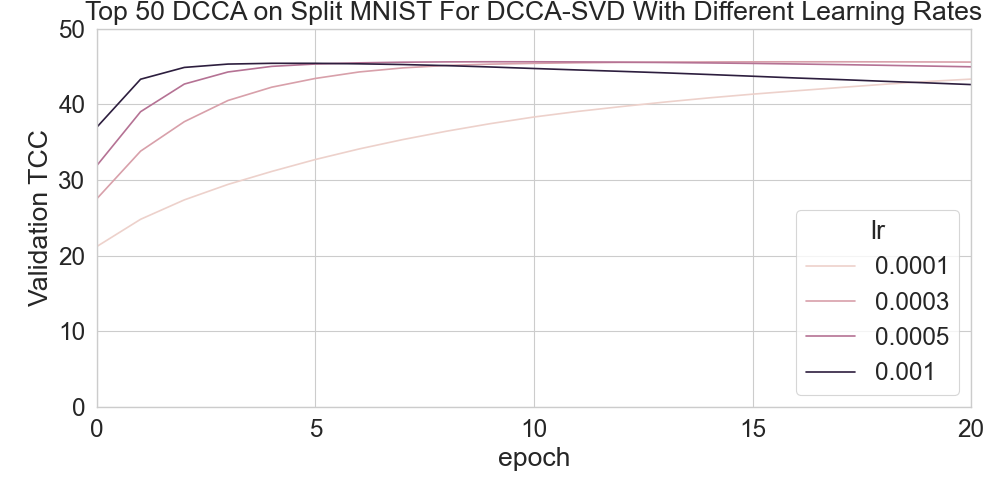
\includegraphics[width=\textwidth]{figures/deep_learning/DCCA/dcca_lr_experiment.png}
         \caption{}
         \label{fig:lrexp}
     \end{subfigure}
     \hfill
     \begin{subfigure}[b]{0.49\textwidth}
         \centering
         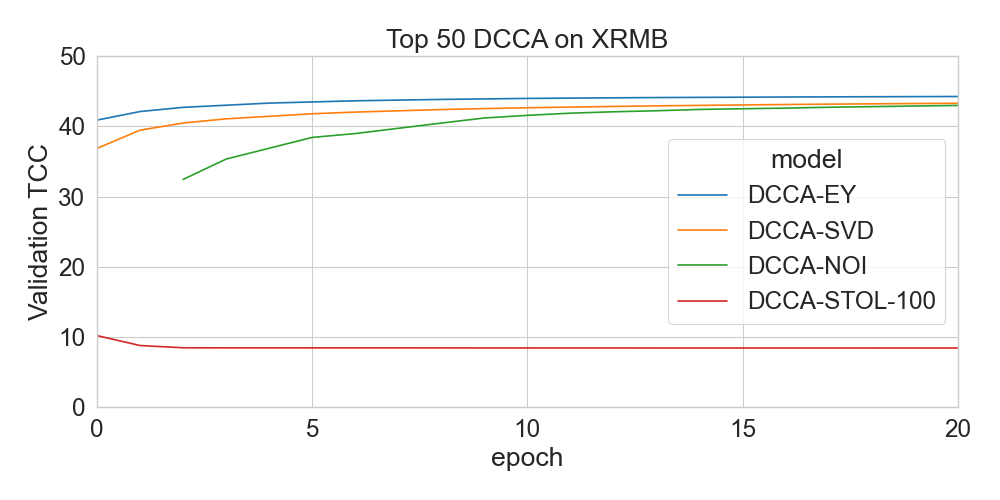
\includegraphics[width=\textwidth]{figures/deep_learning/DCCA/dcca_XRMB.png}
         \caption{}
                 \label{fig:xrmb}
     \end{subfigure}
        \caption{ (a) Validation TCC for different learning rates on Split MNIST data (b) Validation TCC for different methods on XRMB data}

\end{figure}

On the split MNIST data, we show in figure \ref{fig:lrexp} the substantial effect of changing the learning rate on the convergence of the TCC objective. This demonstrates the important of spending computational resource on optimizing the learning rate. An important benefit of our approach is that because the only hyperparameter is learning rate, we can spend all of our computational budget on this critical area. In figure \ref{fig:xrmb}, we show that our proposed methods exhibit extremely fast convergence compared to prior work. Furthermore, both proposed methods find higher validation correlations than DCCA-STOL, showing that they are much more effective ways of estimating the full batch DCCA objective. Note that, the decrease in validation correlation in later epochs is due to overfitting which should be addressed in practical settings by using early stopping as is standard in deep learning.


\subsection{Experiment 2: Application of DCCA-EY to to Deep multiview learning}

%%%%%%%%%%%%%%%%%%%%%%%%%%%%%%%%%%%%%%%%%%%%%%%%%%%%%%%%%%%%%%%%%%%%%%%%%%%%%%%%%%%%%%
%SSL
%%%%%%%%%%%%%%%%%%%%%%%%%%%%%%%%%%%%%%%%%%%%%%%%%%%%%%%%%%%%%%%%%%%%%%%%%%%%%%%%%%%%%%
\subsection{Experiment 3: Application of SSL-EY to Self-Supervised Learning}

In this section, we test our SSL objectives on the CIFAR-10 and CIFAR-100 datasets, which both have 60,000 images and 10 and 100 classes respectively. We compare our methods, SSL-EY and SSL-SVD, with two state-of-the-art methods, Barlow Twins and VICReg. We report k-Nearest Neighbor accuracy on the representations of the validation data in a zero-shot setup.

Firstly, we consider a standard experiment from the literature.
We use the sololearn package \cite{da2022solo}, which includes optimised hyperparameters (and augmentations) for VICReg and Barlow Twins on this specific task.
Each method uses a ResNet-18 encoder, a two-layer projector network with 2048 units in each layer, and is trained for 1,000 epochs with a minibatch size of 256.
For SSL-EY and SSL-SVD, we use the same hyperparameters as Barlow Twins.  
Table \ref{tab:selfsup} shows that our methods are competitive with Barlow Twins and VICReg in this setup.
This is remarkable because their tuning parameters had been heavily optimised, and our method required no tuning at all!

We then performed ablation studies to understand the importance of the (many) hyperparameters in these joint embedding models. In general we found that VICReg was much more sensitive to these hyperparameters than Barlow Twins but that our method was significantly more stable than either of them, see supplement \ref{supp:ablation}.
Table \ref{tab:selfsupsmaller} shows a particularly striking example of this. 
We repeat the previous experiment with all hyperparameters the same apart from the projector: we take a smaller projector with only 256 units in each layer. 
Comparing Tables \ref{tab:selfsup} and \ref{tab:selfsupsmaller} shows that VICReg and Barlow Twins have a large performance drop with the smaller projector on the non-trivial classification problems; our methods are much less affected, and now significantly outperform VICReg and Barlow Twins.
 

\begin{table}[h] 
\centering 
\begin{tabular}{lcccc} 
\hline 
Method & CIFAR-10 Top-1 & CIFAR-10 Top-5 & CIFAR-100 Top-1 & CIFAR-100 Top-5 \\ 
\hline 
Barlow Twins & \textbf{92.1} & 99.73 & \textbf{71.38} & \textbf{92.32}\\
VICReg & 91.68	&99.66 & 68.56&	90.76 \\
\textbf{SSL-EY} & 91.43& \textbf{99.75}& 67.52& 90.17\\
\textbf{SSL-SVD} & 90.57 & 99.71 & 65.93 & 89.31 \\
\hline 
\end{tabular} \caption{SSL methods on CIFAR-10 and CIFAR-100 using 2048 unit projectors.} \label{tab:selfsup}
\centering 
\begin{tabular}{lcccc} 
\hline 
Method & CIFAR-10 Top-1 & CIFAR-10 Top-5 & CIFAR-100 Top-1 & CIFAR-100 Top-5 \\ 
\hline 
Barlow Twins & 88.35 & \textbf{99.71} & 59.94 & 85.99 \\
VICReg & 88.74 & 99.68 & 57.03& 84.45 \\
\textbf{SSL-EY} & 89.49 & 99.54 & \textbf{65.62}& \textbf{89.00}\\
\textbf{SSL-SVD} & \textbf{90.34} & 99.67 & 64.54 & 88.66 \\
\hline 
\end{tabular} \caption{SSL methods on CIFAR-10 and CIFAR-100 using 256 unit projectors.} \label{tab:selfsupsmaller} \end{table}


\subsection{Deep CCA Minibatch Size}

We investigated how the minibatch size affects the performance of DCCA-SVD. As we can see in figure \ref{fig:deep minibatch size ablation}, and consistent with the previous experiments with linear CCA, smaller minibatches can converge much faster on a per-epoch basis. Furthermore, since there is evidence of overfitting on the validation TCC metric, this experiment also demonstrates the need for regularisation in the deep learning setting.  While for this simple problem the issue can be solved by early stopping, it raises interesting questions for the self-supervised learning setting including what we should use as a metric for tuning.

\begin{figure}[h]
\centering
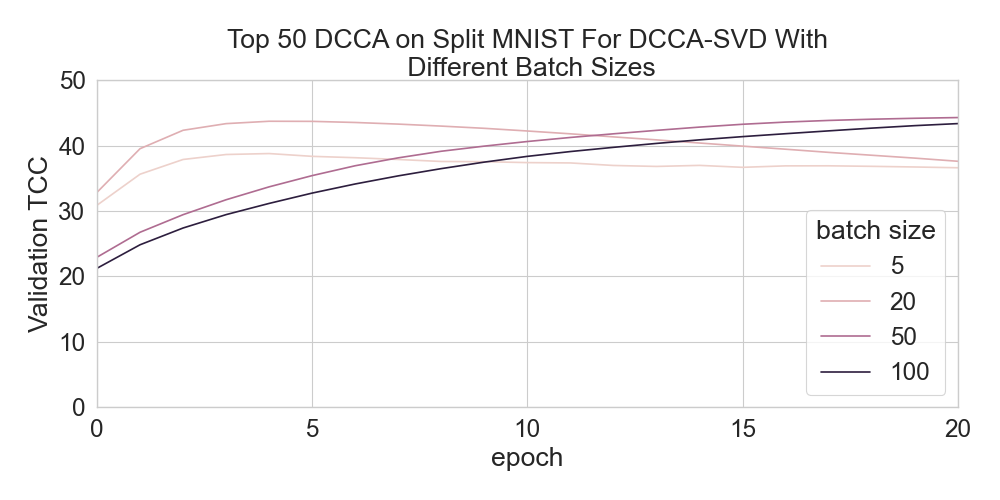
\includegraphics[width=\textwidth]{figures/deep_learning/DCCA/deep_SplitMNIST_minibatch_size_ablation.png}
\caption{}
\label{fig:deep minibatch size ablation}
\end{figure}


\subsection{SSL}
To evaluate the robustness of our proposed method, we conduct ablation studies on different hyperparameters that may affect the performance, including further studies on projector dimensions, removing the projector altogether, different augmentations, and minibatch sizes.

\textbf{Further Projector Sizes}: We ran each model for projector sizes 64, 128, 256, and 2048. As shown in figure \ref{fig:projectorablation}, we found that with our methods performance was surprisingly stable even down to projector size 64. It is worth noting that the performance curves do have a clear `elbow' at projector size 256 for CIFAR-100 while for CIFAR-10 performance is flat even for projector size 64. This could suggest that the natural size of the subspace is of a similar order of magnitude to the number of classes in these particular datasets. 

\begin{figure}[h]
     \centering
     \begin{subfigure}[b]{0.49\textwidth}
         \centering
         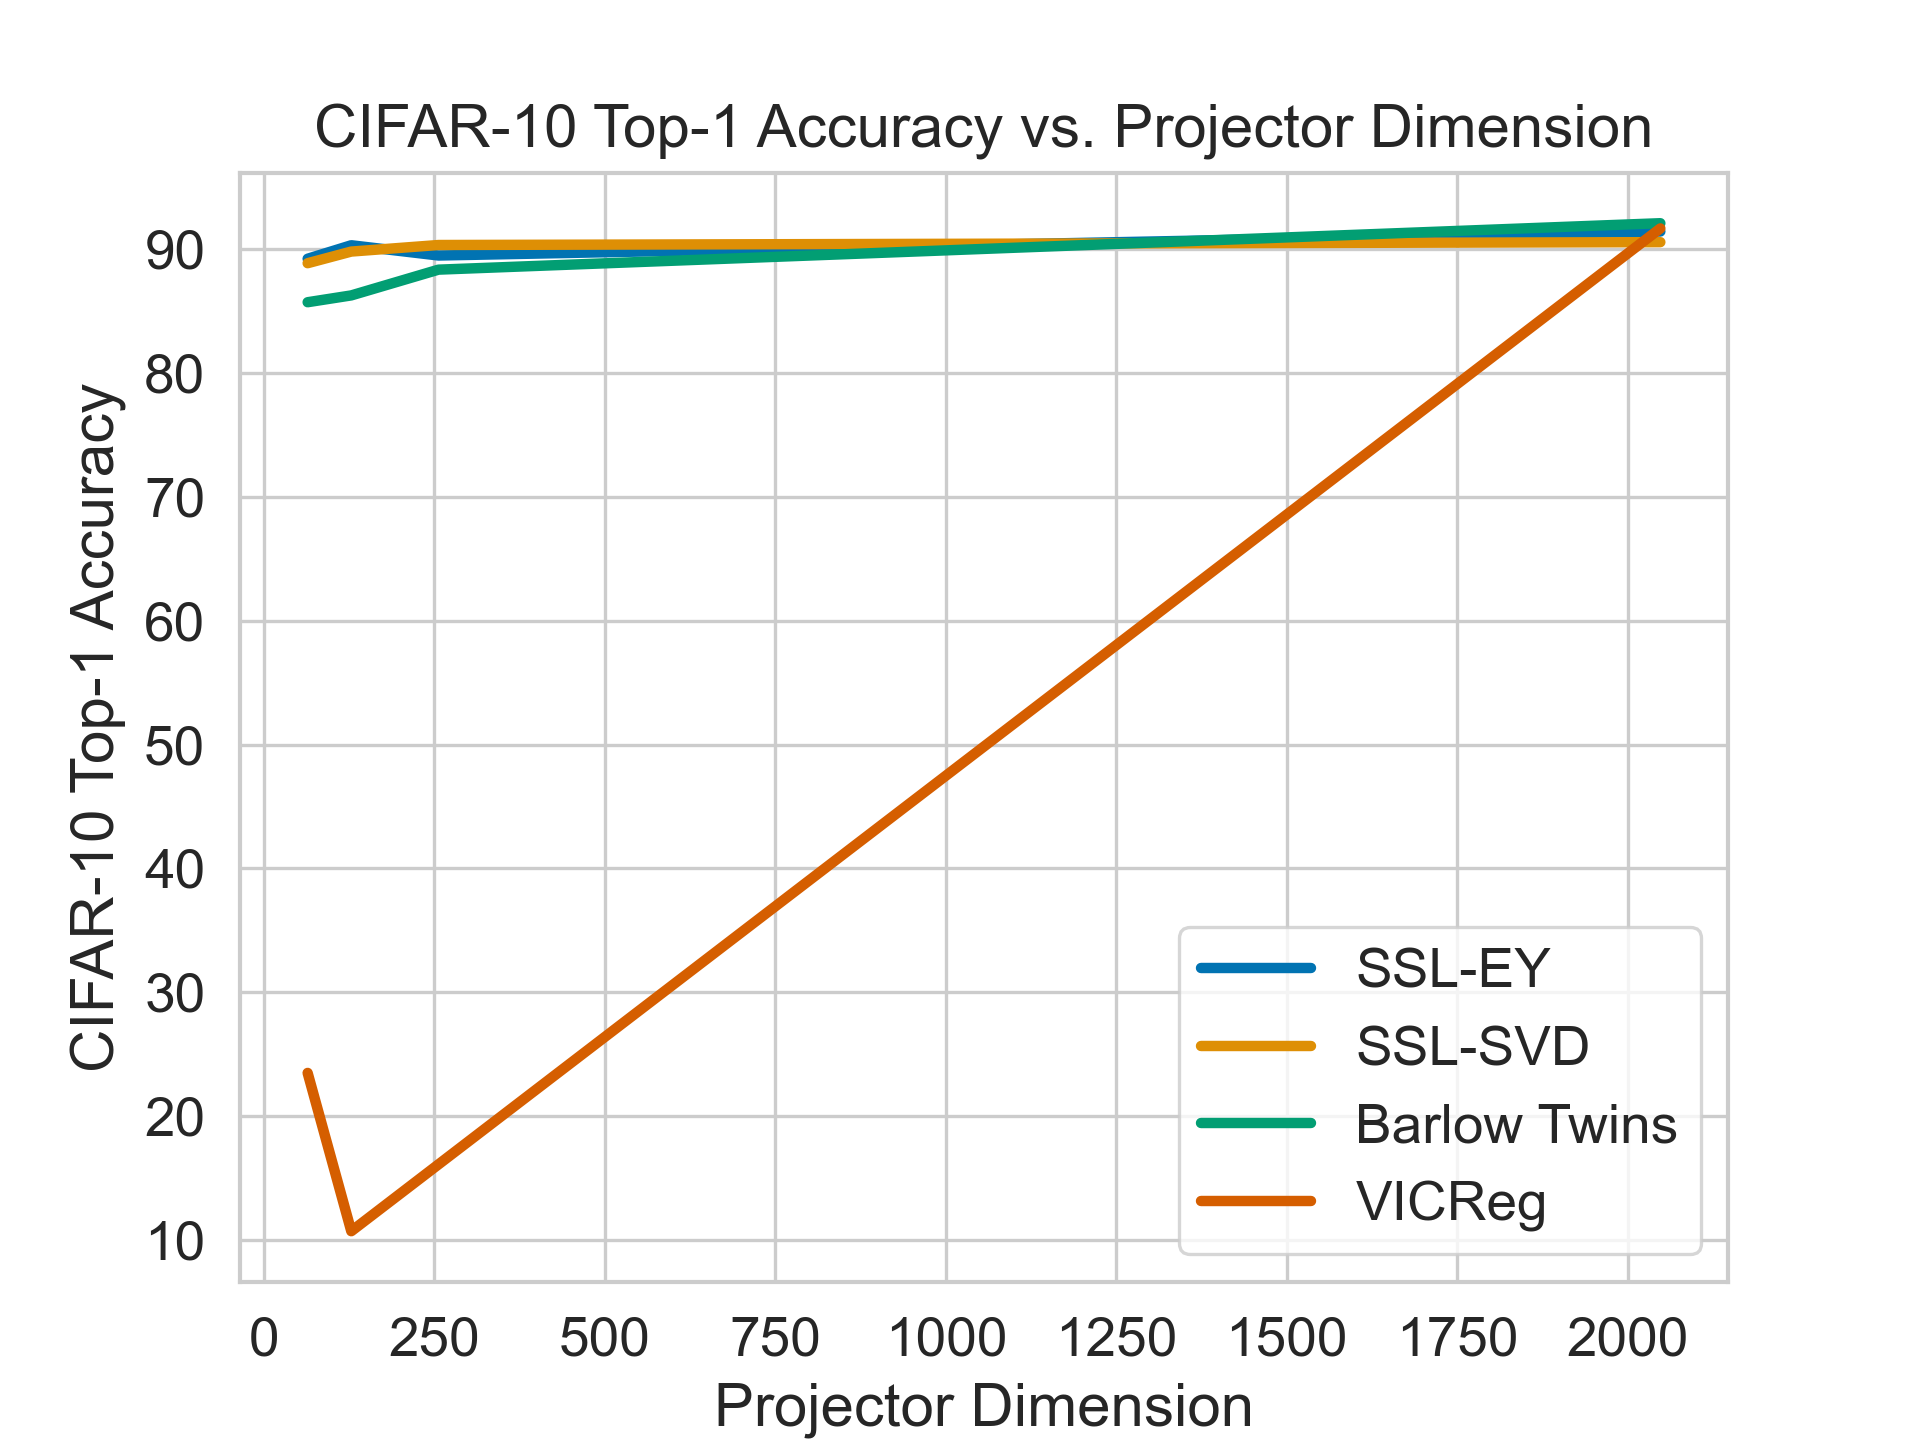
\includegraphics[width=\textwidth]{figures/deep_learning/SSL/cifar10_proj_dim.png}
         \caption{}
         \label{fig:lrexp}
     \end{subfigure}
     \hfill
     \begin{subfigure}[b]{0.49\textwidth}
         \centering
         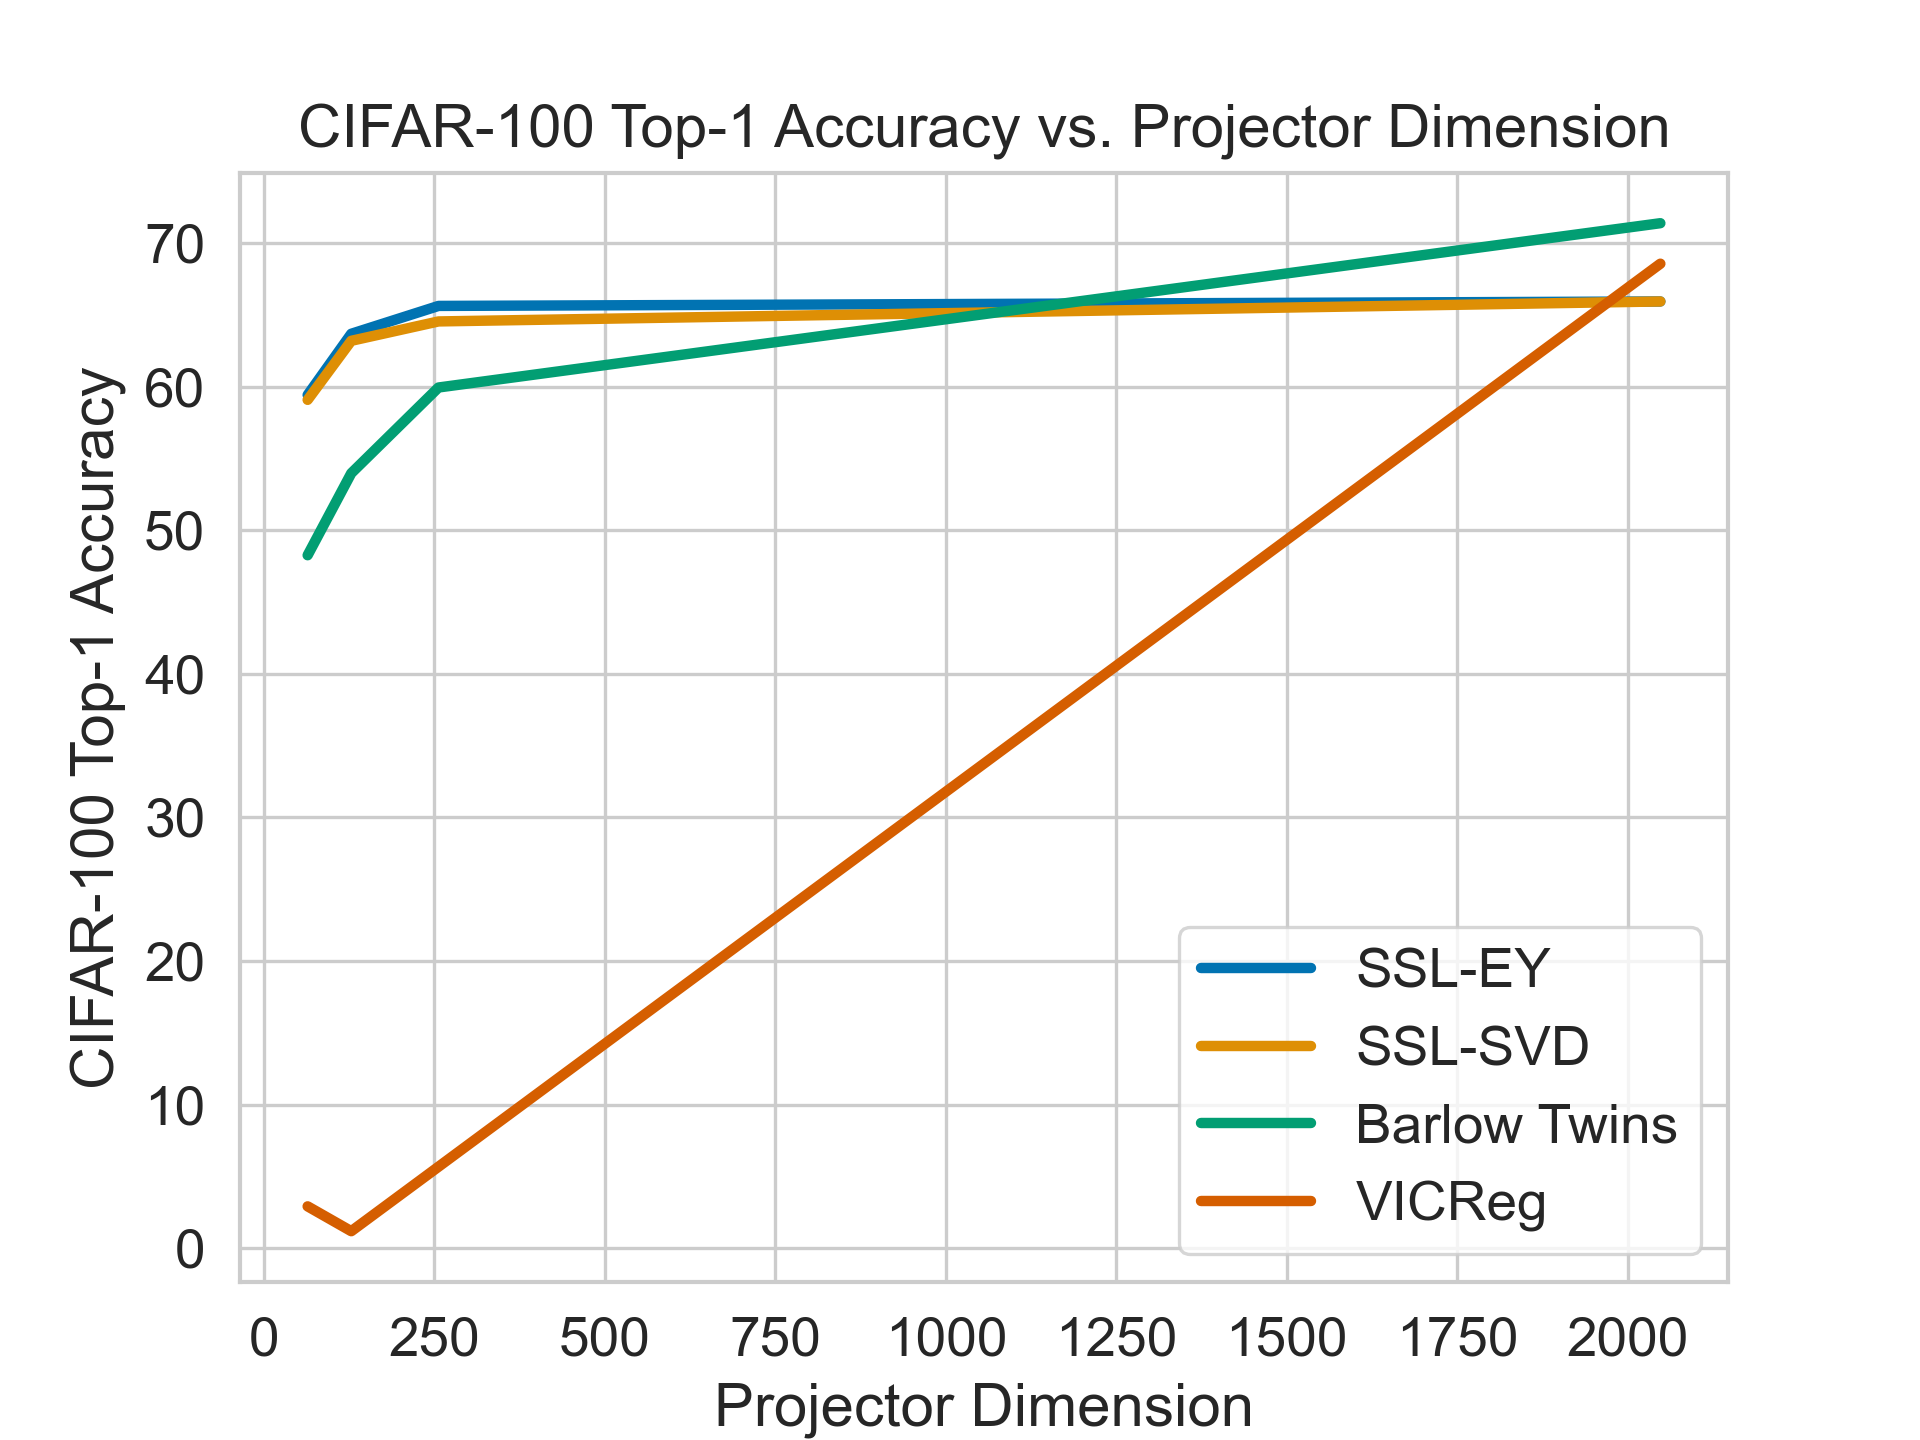
\includegraphics[width=\textwidth]{figures/deep_learning/SSL/cifar100_proj_dim.png}
         \caption{}
                 \label{fig:xrmb}
     \end{subfigure}
        \caption{Performance against projector capacity (a) Top-1 accuracy for CIFAR-10 (b) Top-1 accuracy for CIFAR-100}
    \label{fig:projectorablation}
\end{figure}

\textbf{No Projector}: We conducted an experiment where instead of using the learnt representations from the resnet-18 output for classifications, we used the output of the projector directly with results presented in table \ref{tab:selfsupsmaller}. We make the same observation that the projector doesn't appear to be a neccessary feature of our proposed method with similar performance whether classification is made on the `representations' or `embeddings'. Indeed, our methods perform better than competitors in this setting. Despite the similarities between the motivations of all 4 methods, it is an interesting open question that Barlow twins benefits so much from the use of a projector and our results suggest that it is not a neccessary feature of correlation based models.

\begin{table}[h!] 
% thanks GPT
\setlength{\tabcolsep}{6pt} % sets the padding on left and right of each column
\renewcommand{\arraystretch}{1.1} % increase the row height
\centering 
\begin{tabular}{llcccc} 
\toprule
&& \multicolumn{2}{c}{CIFAR-10} & \multicolumn{2}{c}{CIFAR-100} \\ 
\cmidrule(lr){3-4} \cmidrule(lr){5-6}
Method & Output & Top-1 & Top-5 & Top-1 & Top-5 \\ 
\midrule
Barlow Twins & Encoder & 92.1 & 99.73 & 71.38 & 92.32\\
Barlow Twins & Projector & 89.99&99.21 & 63.51&86.99\\
\midrule
VICReg & Encoder & 91.68	&99.66 & 68.56&	90.76\\
VICReg & Projector & \textbf{90.99}&99.46 & 63.82&86.39\\
\midrule
SSL-EY & Encoder & 89.49 & 99.54 & 65.62& 89.00\\
SSL-EY & Projector & 90.98 &\textbf{99.69} & \textbf{65.21}&\textbf{88.09}\\
\midrule
SSL-SVD & Encoder & 90.34 & 99.67 & 64.54 & 88.66 \\
SSL-SVD & Projector & 90.12& 99.59 & 63.14& 87.51
 \\
\bottomrule
\addlinespace
\end{tabular}
\caption{SSL methods on CIFAR-10 and CIFAR-100 using 256 unit projectors.} 
\label{tab:selfsupsmaller} 
\end{table}

\textbf{Augmentations}: We used VICReg augmentations and Barlow Twins augmentations with each of our proposed methods. We found that performance was similar and therefore confirms that differences in performance across Barlow Twins, VICReg, and our two methods is driven by differences in the objective.

\begin{table}[h!] 
\setlength{\tabcolsep}{6pt} % sets the padding on left and right of each column \renewcommand{\arraystretch}{1.1} % increase the row height 
\centering 
\begin{tabular}{llcccc} 
\toprule 
&& \multicolumn{2}{c}{CIFAR-10} & \multicolumn{2}{c}{CIFAR-100} \\ % added multicolumn for the two datasets 
\cmidrule(lr){3-4} \cmidrule(lr){5-6} % added horizontal lines to separate the columns
Method & Augmentation & Top-1 & Top-5 & Top-1 & Top-5 \\ 
\midrule
SSL-EY & Barlow Twins & 89.49 & 99.54 & 65.62& 89.00\\ 
SSL-EY & VICReg &90.43& 99.62 & 64.34&87.89\\ 
\midrule 
\addlinespace 
SSL-SVD & Barlow Twins & 90.34 & 99.67 & 64.54 & 88.66 \\ 
SSL-SVD & VICReg &89.36& 99.66 & 63.68&87.49 \\ 
\bottomrule 
\addlinespace 
\end{tabular} 
\caption{SSL methods on CIFAR-10 and CIFAR-100 using different augmentations.} 
\label{tab:selfsupsug} 
\end{table}


\textbf{Minibatch Size}: We ran experiments with minibatch sizes ranging from 128 to 512 (noting that this means four times as many iterations for 128 vs 512). Figure \ref{fig:sslbsablation} shows that methods generally performed strongly even as batch size was reduced.

\begin{figure}[h!]
     \centering
     \begin{subfigure}[b]{0.49\textwidth}
         \centering
         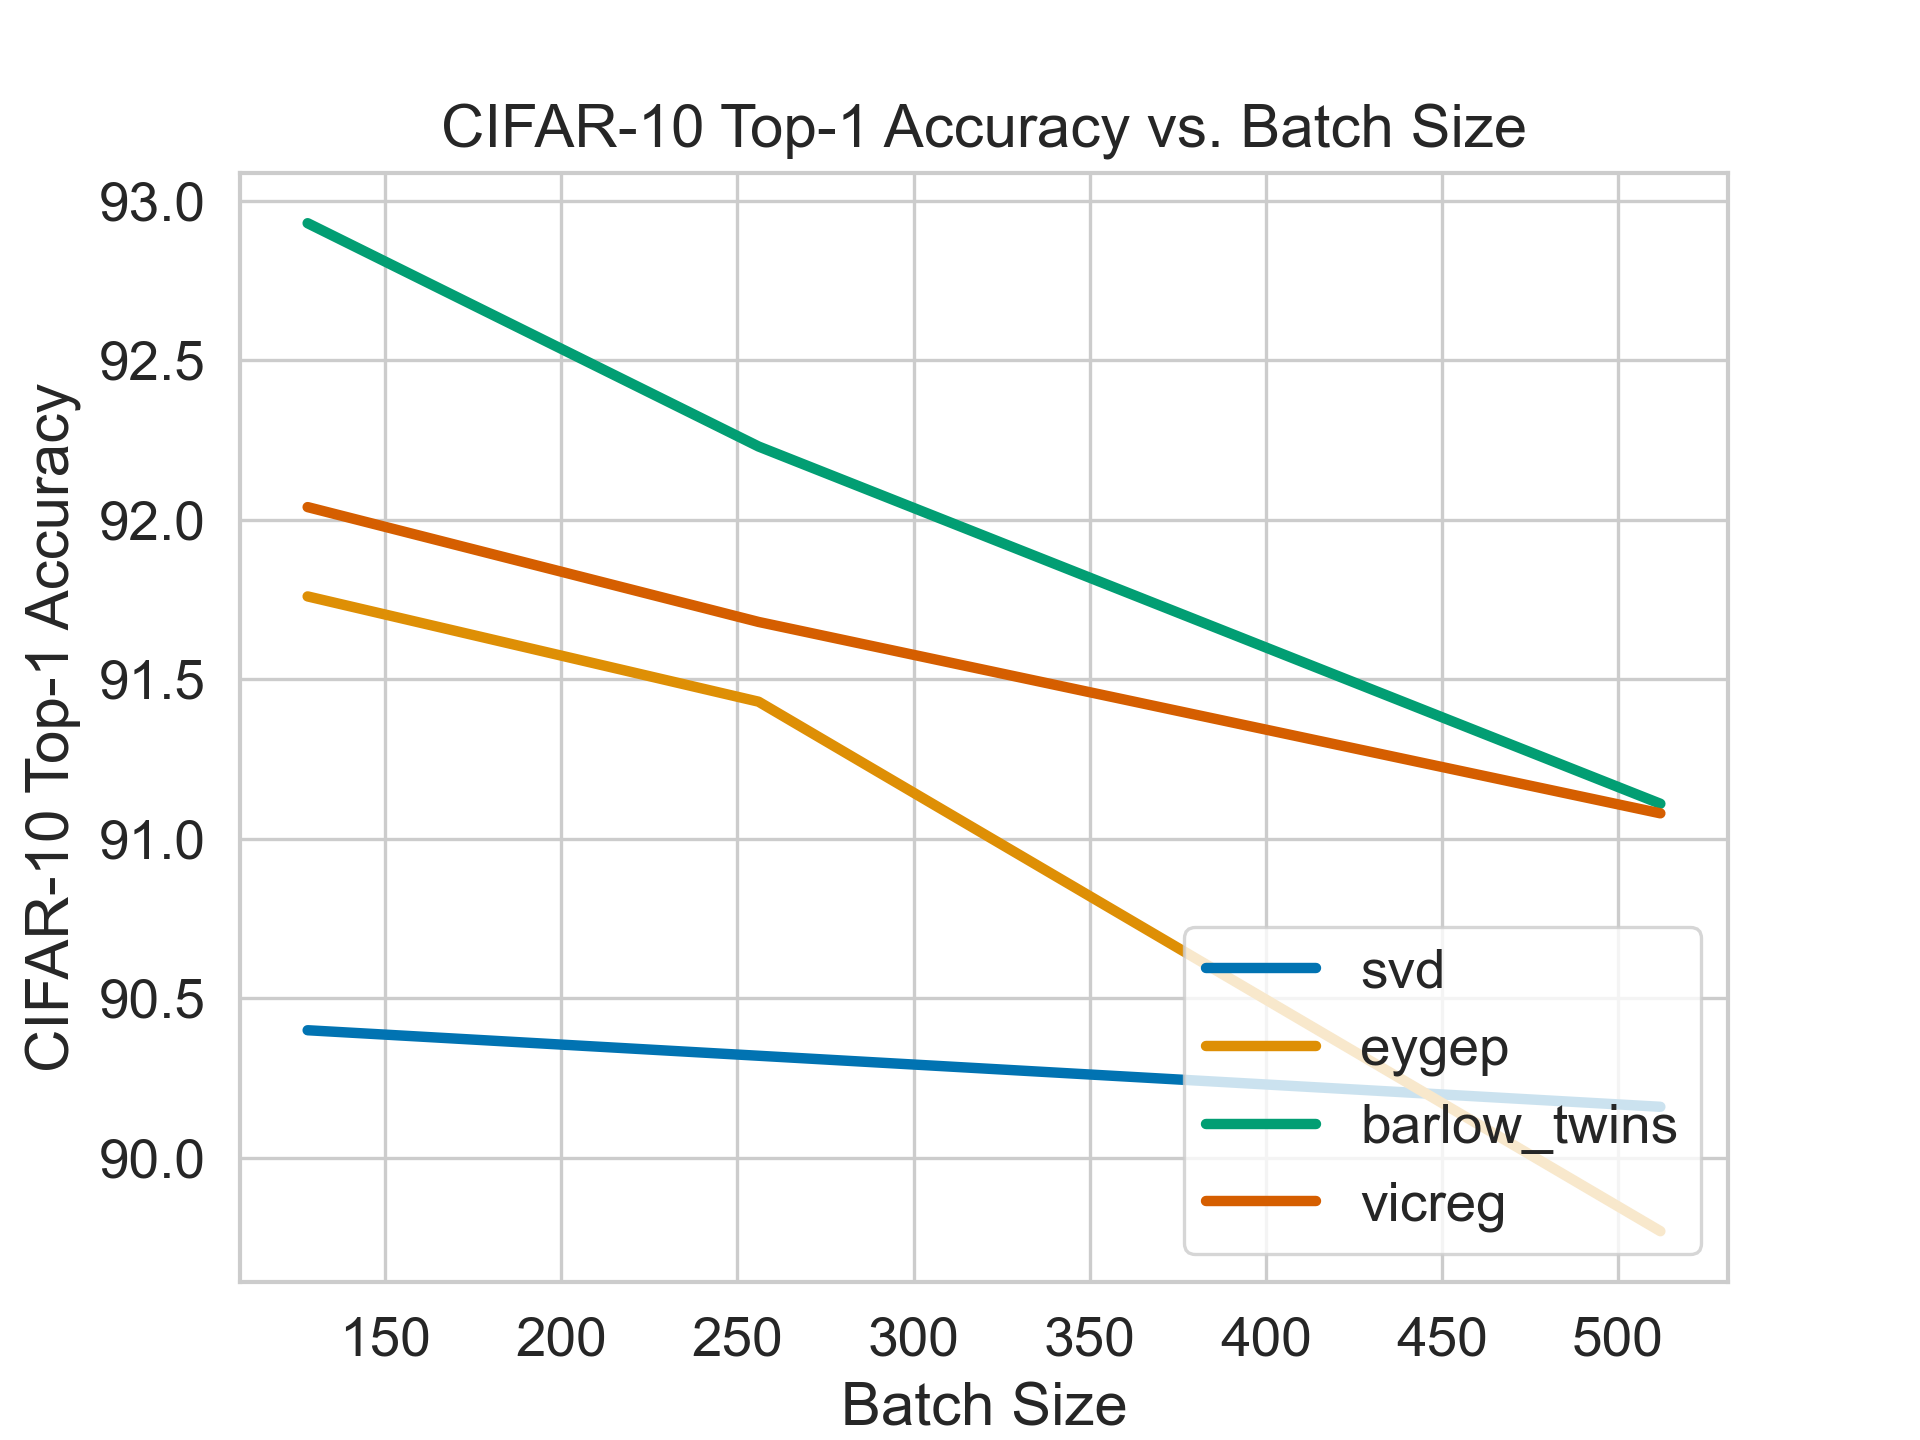
\includegraphics[width=\textwidth]{figures/deep_learning/SSL/cifar10_bs.png}
         \caption{}
         \label{fig:lrexpminibatch}
     \end{subfigure}
     \hfill
     \begin{subfigure}[b]{0.49\textwidth}
         \centering
         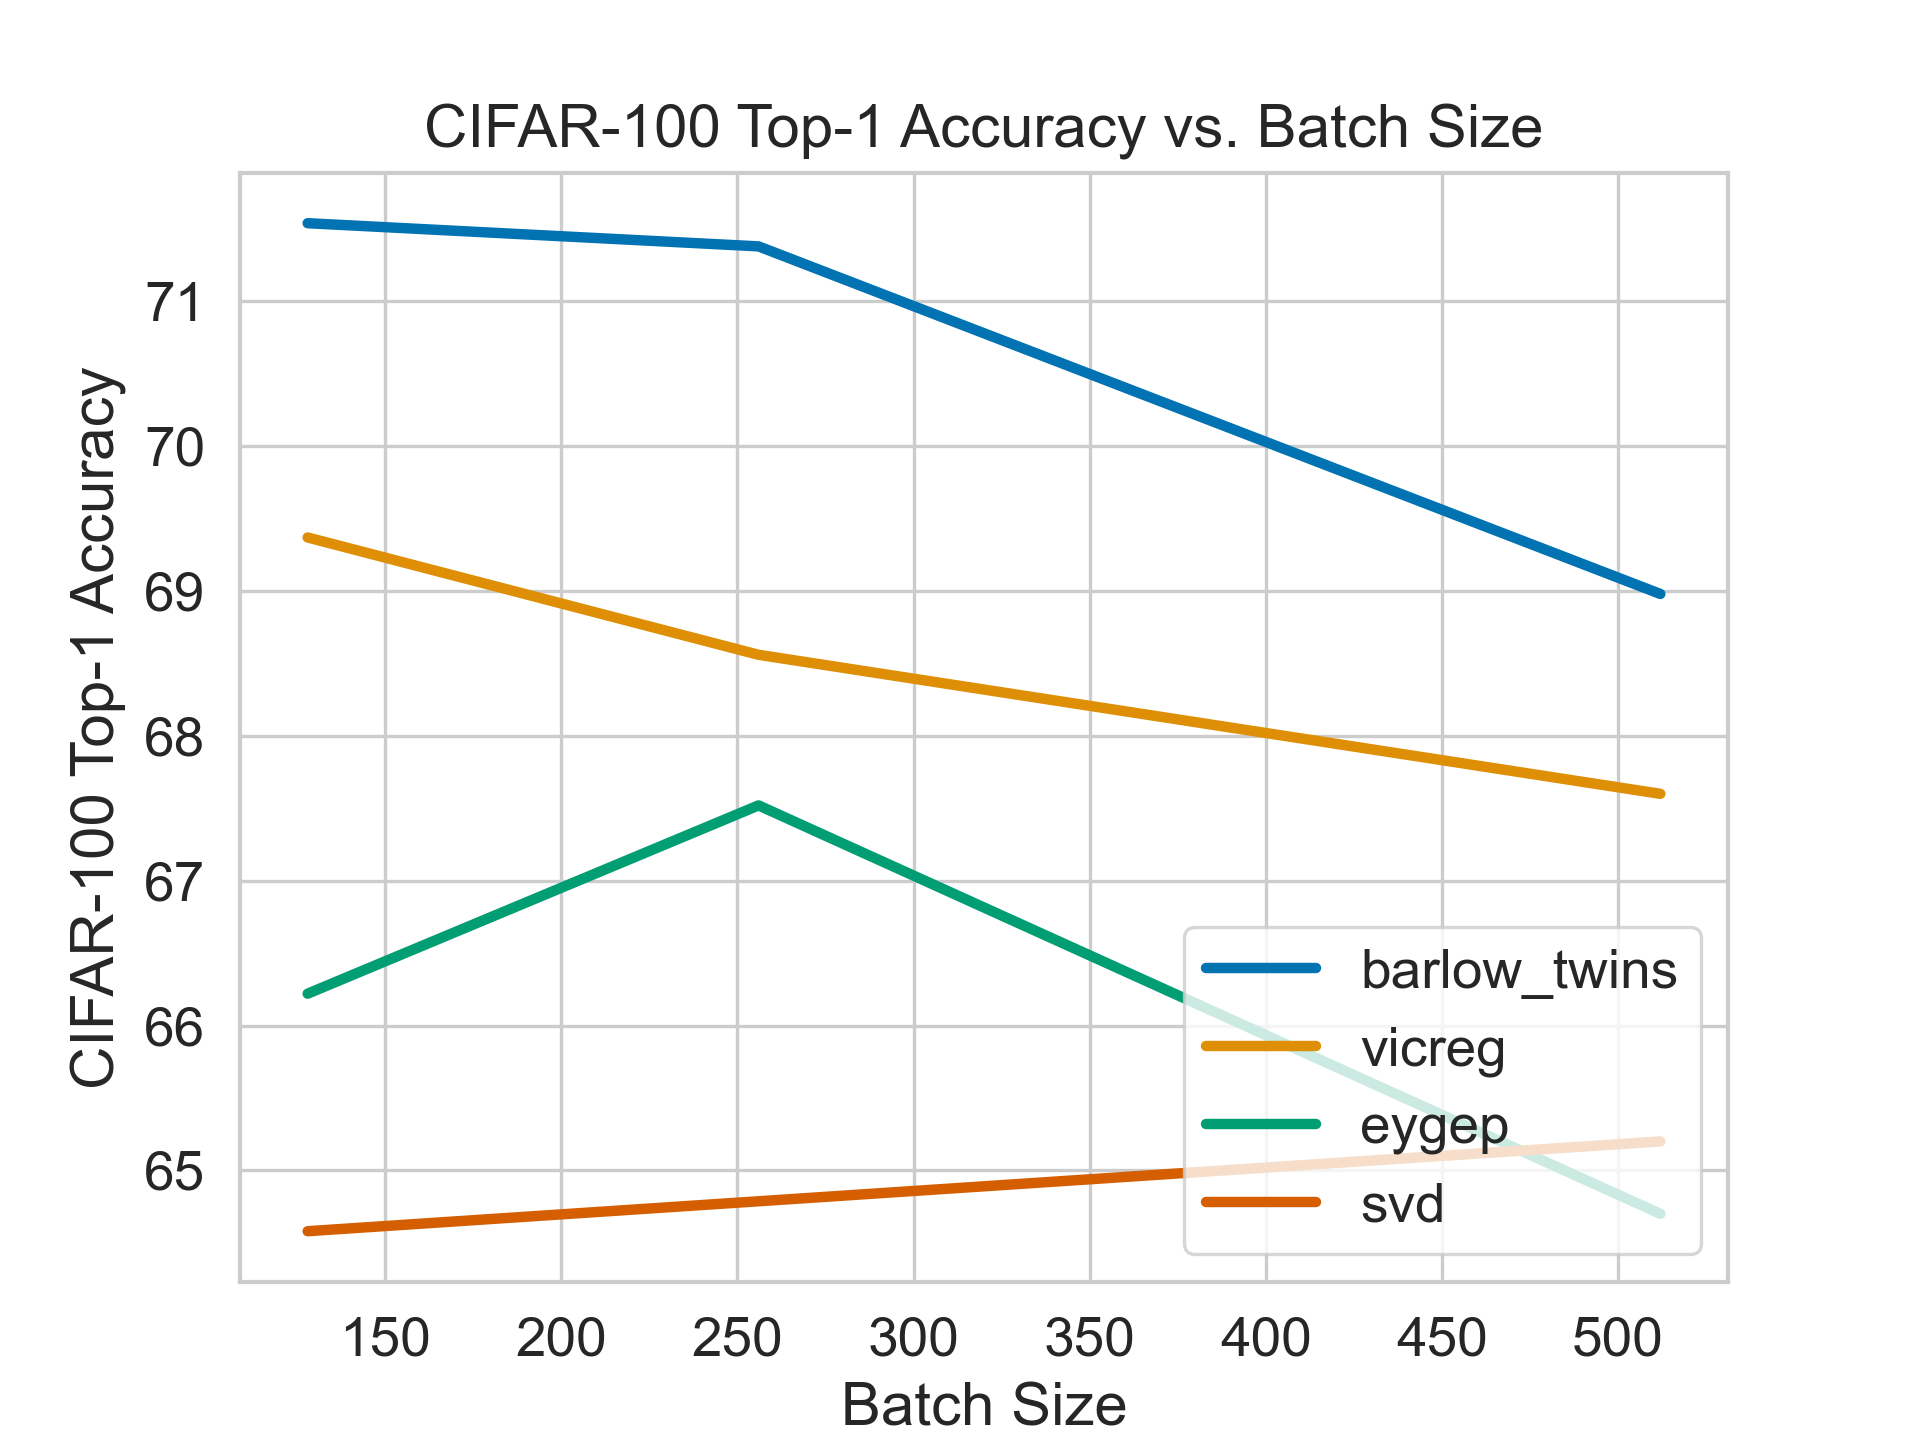
\includegraphics[width=\textwidth]{figures/deep_learning/SSL/cifar100_bs.png}
         \caption{}
                 \label{fig:xrmbminibatch}
     \end{subfigure}
        \caption{Performance against projector capacity (a) Top-1 accuracy for CIFAR-10 (b) Top-1 accuracy for CIFAR-100}
    \label{fig:sslbsablation}
\end{figure}


\section{Discussion and Conclusion}





